\documentclass{article}

\usepackage[paper=letterpaper,margin=2.5cm]{geometry} % Set Margins

%% Math and math fonts
\usepackage{amsmath, amsthm, amssymb, amsfonts}
\usepackage{bbm} % for \mathbbm{1}

% date
\usepackage[nodayofweek]{datetime}

% Color
\usepackage{color, xcolor}

% Misc
\usepackage{environ}  % \collect@body in asmmath
\usepackage{graphicx} % \includegraphics options
\usepackage{mdframed} % text boxes
\usepackage{indentfirst} % Indent first paragraph after section header
\usepackage{comment} % Comments
\usepackage{fancyhdr} % Headers and footers

% Tables
\usepackage{array}

% Sub-figures and figure placement
\usepackage{caption}
\usepackage{subcaption}
\usepackage{float} 

% Graphing
\usepackage{pgfplots}
\pgfplotsset{compat=1.17}
\usepackage{tikz}

% Title Placement
\usepackage{titling}
\setlength{\droptitle}{-6em}

%set indent to 
\setlength{\parindent}{0pt}

% Hyper refs
\usepackage{hyperref}
\hypersetup{
    colorlinks=true,
    linkcolor=blue,
    urlcolor  = blue,
    filecolor=magenta,      
    urlcolor=blue,
    citecolor = blue,
    anchorcolor = blue
}

% % Citation management
\usepackage{natbib}
\bibliographystyle{abbrvnat}
\setcitestyle{authordate,open={(},close={)}}

\pagestyle{fancy}

\usepackage[paper=letterpaper,margin=2.5cm]{geometry} % Set Margins

%% Math and math fonts
\usepackage{amsmath, amsthm, amssymb, amsfonts}
\usepackage{bbm} % for \mathbbm{1}

% date
\usepackage[nodayofweek]{datetime}

% Color
\usepackage{color, xcolor}

% Misc
\usepackage{environ}  % \collect@body in asmmath
\usepackage{graphicx} % \includegraphics options
\usepackage{mdframed} % text boxes
\usepackage{indentfirst} % Indent first paragraph after section header
\usepackage{comment} % Comments
\usepackage{fancyhdr} % Headers and footers

% Tables
\usepackage{array}

% Sub-figures and figure placement
\usepackage{caption}
% \usepackage{subcaption}
\usepackage{float} 

% Graphing
\usepackage{pgfplots}
\pgfplotsset{compat=1.17}
\usepackage{tikz}

% Title Placement
\usepackage{titling}
\setlength{\droptitle}{-6em}

%set indent to 
\setlength{\parindent}{0pt}

% Hyper refs
\usepackage{hyperref}
\hypersetup{
    colorlinks=true,
    linkcolor=blue,
    urlcolor  = blue,
    filecolor=magenta,      
    urlcolor=blue,
    citecolor = blue,
    anchorcolor = blue
}

% % Citation management
\usepackage{natbib}
\bibliographystyle{abbrvnat}
\setcitestyle{authordate,open={(},close={)}}

\newcolumntype{M}{>{$}c<{$}} % Define a new column type for math mode


% ----------------------------------------
% TITLE
% ----------------------------------------

\pagestyle{fancy}

\lhead{Creel}
\chead{Eigenvalues and eigenvectors}
\rhead{AMES}

\title{AMES Week 12 class notes -- Weds, Eigenvalues and Eigenvectors }
\author{Andie Creel}

\begin{document}
\maketitle

\section{Summary}

Eigenvalues and eigenvectors are fundamental concepts in linear algebra, with applications in various fields such as physics, computer science, and engineering.

\subsection{Eigenvalues and Eigenvectors}

\textbf{Definition:}

\begin{itemize}
  \item \textbf{Eigenvalue (\(\lambda\)):} For a square matrix \(A\), a scalar \(\lambda\) is considered an eigenvalue if there exists a non-zero vector \(q\) such that \(Aq = \lambda q\).
  
  \item \textbf{Eigenvector (\(q\)):} A non-zero vector \(q\) is an eigenvector corresponding to the eigenvalue \(\lambda\) if \(Aq = \lambda q\).
\end{itemize}

\textbf{Eigenvalue Equation:}

The relationship \(Aq = \lambda q\) can be expressed as \((A - \lambda I) q = 0\), where \(I\) is the identity matrix.\\

\textbf{Characteristic Polynomial:}

The characteristic polynomial of \(A\) is given by \(\text{det}(A - \lambda I) = 0\). Solving this equation yields the eigenvalues of \(A\).

\subsection{Interpretation}

The \textbf{eigenvalue} gives you "speed" of the dynamics around an equilibrium. Is a a system going to approach equilibrium's, or move away? Is it happening fast or slow?\\

\begin{itemize}
    \item If all eigen values are positive, the equilibrium is unstable. The system will move away from the equilibrium is perturbed.  
    \item If all eigen values are negative, the equilibrium is stable. The system will move towards the equilibrium if perturbed. 
    \item If one is positive, and the other is negative, it's conditionally stable.
    \item If in eigen value has an imaginary number in it $i = \sqrt{-1}$ such that $\lambda = R + Zi$ that means we have a spiraling equilibrium. If $R$ is positive is spirals out, if $R$ is negative it spirals in. 
\end{itemize}

The \textbf{eigenvector} tells us about the "direction" of the dynamics around the equilibrium. So if you're thinking about populations, it'll tell you how many more or less of a different species you're getting. If you're thinking about the economy, it'll tell you how the share of the economy is going to be split across different industries.


\section{Review of solving for eigenvectors}
Recall from last class, when we consider how the stocks in a system are changing we end up with an equation 
\begin{align}
    (A - \lambda I) q = 0 
\end{align}

where $A$ is the the Jacobian matrix and $q$ is our eigen vector. 

\begin{align}
    (A - \lambda I ) q = 0 \\
    \begin{bmatrix}
        a_{11} - \lambda & a_{12} \\
        a_{21} & a_{22} - \lambda
    \end{bmatrix}
    \begin{bmatrix}
        q_1 \\
        q_2
    \end{bmatrix} = 0 \\
    \implies (a_{11} - \lambda) q_1 + a_{12} q_2 = 0 \label{system_1} \\
    a_{21} q_1 + (a_{22} - \lambda) q_2 = 0 \label{system_2}
\end{align}

The $q$ is only defined relative to another. Conditioned on a given $\lambda$, there is a $q_2$ for any $q_1$ that solves this system. \\

So we will say the eigen vector is length 1 for convenience. This sets up the equation 
\begin{align}
    q_1^2 + q_2^2 = 1 \label{pythag}
\end{align}

This then gives us 3 equations (eqn \ref{system_1}, \ref{system_2}, and \ref{pythag})  and 3 unknowns ($q_1, q_2, \lambda).$ We can solve this system of equations for the eigen value $\lambda$ and the eigen vector $\begin{bmatrix}
    q_1\\
    q_2
\end{bmatrix}$.

\section{Variance and covariance}

Consider a matrix of data $M$ with a column for $x$ and column for $y$. \\

Our variance and covariance matrix would be 
\begin{align}
    \begin{bmatrix}
        \sigma_x^2 & \sigma_x^2 \sigma_y^2\\
        \sigma_y^2\sigma_x^2 & \sigma_y^2
    \end{bmatrix} \label{cov}
\end{align}

where 
\begin{align}
    \sigma_x^2 = Var_x(M) = \frac{1}{N} \sum_N (x_i - \bar x) ^2\\
    \sigma_y^2 = Var_y(M) = \frac{1}{N} \sum_N (y_i - \bar y) ^2\\
    \sigma_{xy} = \sigma_{yx} = Cov(x,y) = \frac{1}{N} \sum_N (x_i - \bar x)(y_i - \bar y).
\end{align}

We could rescale our data so that the mean is zero, \textit{i.e.} $\bar x = 0$ and $\bar y = 0 $ and all our equations would simplify. 
\begin{align}
    \sigma_x^2 = Var_x(M) = \frac{1}{N} \sum_N x_i ^2\\
    \sigma_y^2 = Var_y(M) = \frac{1}{N} \sum_N y_i ^2\\
    \sigma_{xy} = \sigma_{yx} = Cov(x,y) = \frac{1}{N} \sum_N x_i y_i.
\end{align}

Instead of using summations to find covariance and variance, we could use linear algebra to get the covariance matrix. Remember that $x$ and $y$ would be $N \times 1$ and $M$ would be $N \times 2$
\begin{align}
    Var(x) = x^T x \\
    Var(y) = y^T y\\
    Cov(M) = M^T M
\end{align}

where $Var(x)$ and $Var(y)$ are scalars and $cov(M)$ is the $2 \times 2$ covariance matrix in eqn \ref{cov}. \\

If we had a 


\section{Principal Components Analysis (PCA)}

\textbf{Principal Components Analysis (PCA)} is a statistical technique used to reduce the dimensionality of a dataset while retaining as much variance as possible. It does this by transforming the original variables into a new set of uncorrelated variables called \textit{principal components}.

\subsection*{Steps of PCA}

\begin{enumerate}
    \item \textbf{Center the Data}: Subtract the mean of each variable to center the dataset at the origin.
    \item \textbf{Compute the Covariance Matrix}: Calculate the covariance matrix of the centered data to understand the relationships between variables.
    \item \textbf{Eigen Decomposition}: Compute the eigenvalues and eigenvectors of the covariance matrix.
    \begin{itemize}
        \item \textit{Eigenvectors}: Represent the directions of the principal components.
        \item \textit{Eigenvalues}: Represent the variance captured by each principal component.
    \end{itemize}
    \item \textbf{Select Principal Components}: Order the eigenvectors by their corresponding eigenvalues (from largest to smallest). The eigenvectors with the largest eigenvalues are the principal components that explain the most variance.
    \item \textbf{Project the Data}: Transform the data into the space defined by the selected principal components, reducing the dimensionality if desired.
\end{enumerate}

The PCA creates a lower dimension dataset that is made of variables that are linear combinations of variables in the original dataset. This preserves the variation in the original dataset, while lowering the dimension of the new dataset. 

\subsection*{Relation to the Covariance Matrix}

The covariance matrix plays a central role in PCA because it quantifies the relationships between variables:
\begin{itemize}
    \item The covariance matrix \( M \) is an \( k \times k\) matrix for \( k \) variables, where the entry \( \sigma_{ij} \) represents the covariance between the \( i \)-th and \( j \)-th variables.
    \item PCA finds the \textit{eigenvectors} of the covariance matrix, which correspond to the directions of maximum variance in the data.
    \item The \textit{eigenvalues} of the covariance matrix measure how much variance is captured along each eigenvector (principal component).
\end{itemize}

\subsection*{Why the Covariance Matrix?}

The covariance matrix encapsulates the structure of the data, such as:
\begin{itemize}
    \item How much variance each variable contributes.
    \item The relationships (correlations) between variables.
\end{itemize}

By analyzing the eigenvectors and eigenvalues of the covariance matrix, PCA identifies the directions (principal components) that maximize variance, allowing dimensionality reduction while preserving as much information as possible.\\


In this course, you don't need to memorize how to do this. But it's good to understand what a principle components analysis is. A PCA determines what are the main variables (principle components) that drive results may be. 

\section{Graph analysis}

\begin{figure}[htp]
    \centering
    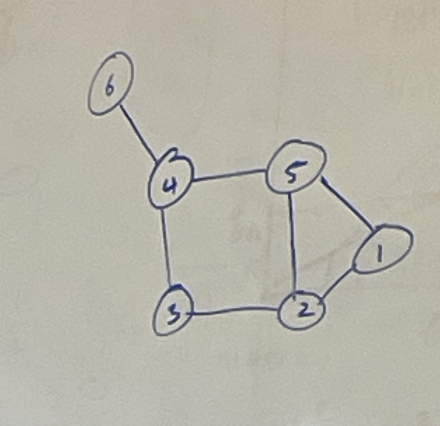
\includegraphics[width=0.5\linewidth]{Screen Shot 2023-11-29 at 11.37.38 AM.png}
    \caption{Graph}
    \label{fig:enter-label}
\end{figure}

With a graph, we can make a \textbf{degree matrix}, which is the number of connections each node has. It's a diagonal matrix. We can make an \textbf{adjacency matrix} so we see which nodes are connected to which. And we could make a \textbf{laplacion matrix} which would be the degree matrix minus the adjacency which tells us about the "speed" of movement between nodes. \\

The adjacency matrix of a graph is a square matrix that represents the connections between vertices. For an undirected graph, the adjacency matrix is symmetric. The \textit{eigenvalues and eigenvectors of the adjacency matrix} provide insights into the graph's connectivity. The \textit{eigenvalues of the Laplacian matrix} are closely related to the number of connected components in a graph. The multiplicity of the eigenvalue in the Laplacian matrix is equal to the number of connected components in the graph. The corresponding eigenvectors provide information about the connectivity within each connected component.\\

Again, you don't need to know all this for this class, but know that it exists. 

\begin{figure}[htp]
    \centering
    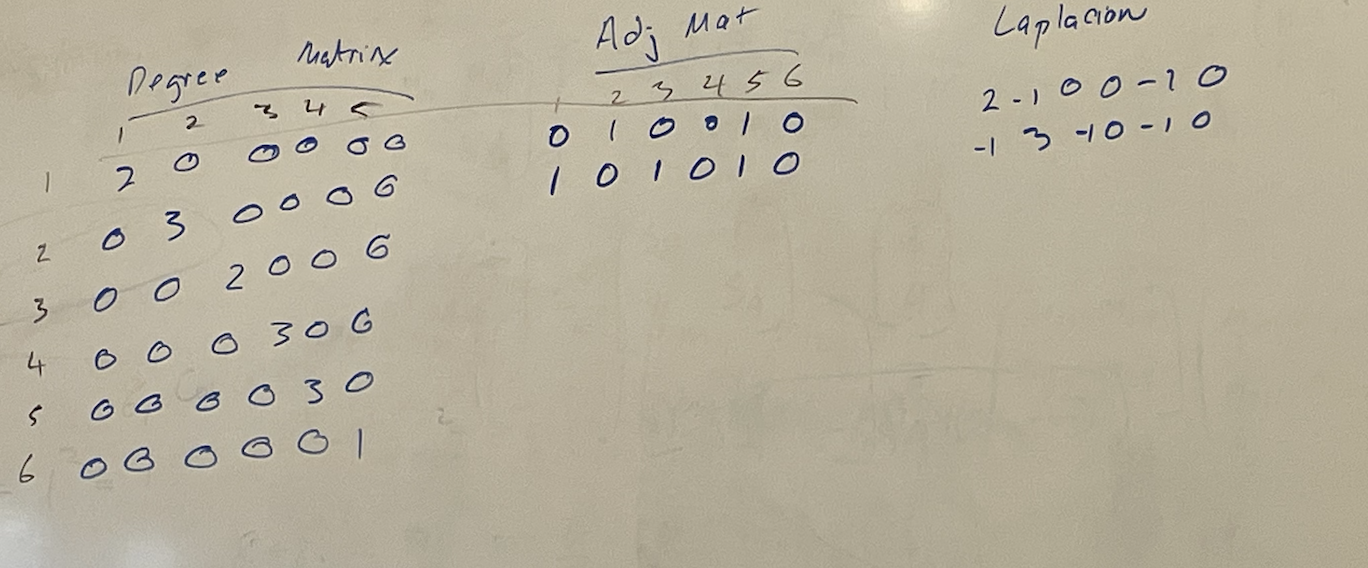
\includegraphics[width=0.75\linewidth]{Screen Shot 2023-11-29 at 11.45.06 AM.png}
    \caption{The matrices}
    \label{fig:enter-label}
\end{figure}





\end{document}